\documentclass[11pt,a4paper]{article}

\usepackage[utf8]{inputenc}
\usepackage[T1]{fontenc}
\usepackage{lmodern}
\usepackage[french]{babel}
\usepackage[margin=2.1cm]{geometry}
\usepackage{microtype}
\usepackage{booktabs}
\usepackage{array}
\usepackage[table]{xcolor}
\usepackage{graphicx}
\usepackage{caption}
\usepackage[most]{tcolorbox}

\definecolor{navy}{HTML}{1F3864}
\definecolor{bluemid}{HTML}{2E5496}
\definecolor{lightblue}{HTML}{D6E0F0}
\definecolor{accent}{HTML}{C0491F}

\captionsetup{font=small,labelfont={bf,color=navy},labelsep=period}
\graphicspath{{../../vasicek_lab/figures/}}

\newtcolorbox{cle}[1][]{colback=lightblue!40,colframe=navy,boxrule=0.6pt,
  arc=2pt,left=8pt,right=8pt,top=6pt,bottom=6pt,#1}

\title{\vspace{-1.2cm}\color{navy}\bfseries Cas d'usage : pilier 2, gestion des incidents\\[2pt]
  \large Du score de criticité à quelques KPI mesurables}
\author{Kélian Kaddouri}
\date{\today}

\begin{document}
\maketitle
\vspace{-0.7cm}

\begin{cle}
\textbf{Pourquoi ce cas d'usage.} Deux praticiens le confirment : la contagion dirigée
entre piliers ($W$) n'est pas identifiable sur donnée réelle. C'est le verdict chiffré du
script de faisabilité (placebo, $z \approx -0{,}1$), rejoint par le jugement métier de
M.~Cherkaoui. La cascade \textbf{reste le modèle normatif} (jugement d'expert assumé,
analyse de sensibilité) ; on met le poids \textbf{empirique} là où la donnée existe.
Choix retenu : \textbf{P2, gestion des incidents}, sur donnée open source, avec pour but
de \textbf{traduire le score de criticité en KPI}.
\end{cle}

\subsection*{Définir l'incident significatif : deux lentilles}

Un incident déclenche l'obligation de gestion P2 s'il est \textbf{significatif}. Deux
lectures complémentaires, chacune adossée à une source :
\begin{itemize}\itemsep2pt
\item \textbf{impact financier} : perte en euros au-dessus d'un seuil (SAS OpRisk) ;
\item \textbf{impact réputationnel} : révélation publique et médiatisation (Data Breach
      Chronology).
\end{itemize}
Elles ne sélectionnent pas les mêmes incidents : un rançongiciel payé discrètement pèse
en euros sans presse, une fuite de données pèse en presse sans perte directe. La maille
P2 doit unir les deux, ce qui justifie un \textbf{score} plutôt qu'un simple montant.

\begin{center}
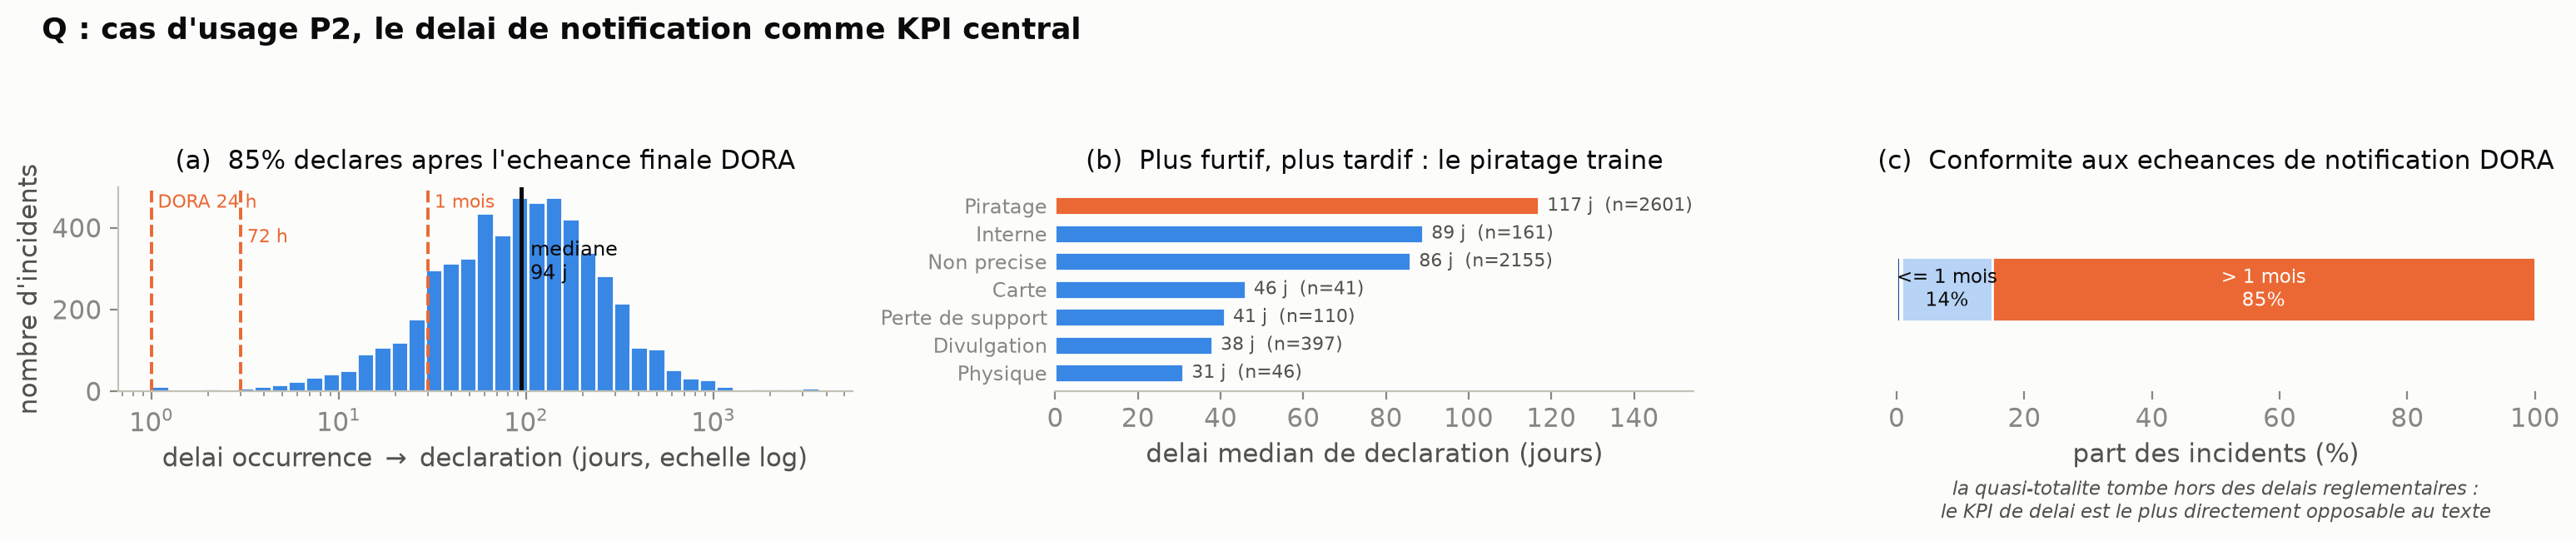
\includegraphics[width=\linewidth]{Q_cas_usage_p2.png}
\captionof{figure}{Socle empirique du cas P2 (secteur financier, Data Breach Chronology).
Le \textbf{délai de notification} est le KPI le plus directement opposable à DORA :
médiane de 94 jours, \textbf{85\,\% des incidents déclarés après l'échéance finale d'un
mois}. Il croît avec la furtivité (piratage 117 j contre incident physique 31 j).}
\end{center}

\subsection*{Traduire le score en KPI (la demande de M.~Cherkaoui)}

Le modèle donne une criticité $=$ f(probabilité, gravité). Pour P2, chaque facteur se lit
comme une quantité \textbf{observable} :

\begin{center}\small
\renewcommand{\arraystretch}{1.25}
\begin{tabular}{@{}l l l l@{}}
\toprule
\textbf{KPI} & \textbf{Valeur} & \textbf{Lecture DORA / métier} & \textbf{Source} \\
\midrule
Fréquence d'incidents & $0{,}10$ à $0{,}21$ / entité / an & probabilité d'occurrence & 08b (OpRisk) \\
Impact financier (queue) & indice $\xi \approx 0{,}90$ & gravité, queue lourde & 05 (OpRisk) \\
\textbf{Délai de notification} & \textbf{médiane 94 j ; 85\,\% $>$ 1 mois} & conformité art.~19 DORA & 08e (Breach) \\
Difficulté de détection & piratage 117 j / physique 31 j & délai selon furtivité & 08e (Breach) \\
Accumulation tiers & 20\,\% portés par causes communes & concentration (P4) & 08d (Breach) \\
\bottomrule
\end{tabular}
\end{center}

\begin{cle}
\textbf{Le score abstrait devient un tableau de bord de quatre quantités observables.} La
\emph{probabilité} du modèle s'incarne dans la \textbf{fréquence} ; la \emph{gravité} dans
l'\textbf{impact financier} et le \textbf{délai de notification} ; et l'accumulation par
cause commune (un tiers qui tombe, plusieurs entités touchées) rejoint le pilier P4, que
M.~Cherkaoui désigne comme le point d'entrée le plus critique. Le délai est le plus
précieux : personne ne le regarde sans la donnée, et il est directement opposable au
texte réglementaire.
\end{cle}

\vspace{-0.1cm}
\noindent\footnotesize\textcolor{navy}{\textbf{Caveats assumés.}} (1)~\texttt{reported\_date}
est la révélation \emph{publique} (notification d'État américain), pas la notification au
superviseur au sens DORA : le délai mesuré est un \textbf{majorant illustratif}, valable
pour comparer les types entre eux, non une mesure du délai réglementaire. (2)~Donnée
\textbf{américaine}, proxy d'entités soumises à DORA. (3)~La tendance annuelle du délai est
biaisée par la troncature à droite (un incident récent n'apparaît que s'il est déjà
déclaré) : non présentée comme résultat. Figure produite par \texttt{08e\_cas\_usage\_p2.py}.

\end{document}
